%%%%%%%%%%%%%%%%%%%%%%%%%%%%%%%%%%%%%%%%%%%%%%%%%%%%%%%%%%%%%%%%%%%%%%
% This layout was adapted from one found at latextemplates.com which
% was adapted from another.
%
% License: CC BY-NC-SA 3.0
% (http://creativecommons.org/licenses/by-nc-sa/3.0/)
%
% Original header:
%
% This is a LaTeX version of the sample laboratory report from
% Virginia Tech's copyrighted 08-09 CHEM 1045/1046 lab manual.
% Reproduction of this one appendix section for academic purposes
% should fall under fair use.
%
%%%%%%%%%%%%%%%%%%%%%%%%%%%%%%%%%%%%%%%%%%%%%%%%%%%%%%%%%%%%%%%%%%%%%%

\documentclass{article}

\usepackage{graphicx} % Lets us use images
%\usepackage[acronym]{glossaries} % Lets us use acronyms
\usepackage{multicol}
\usepackage{subcaption}

\author{Charles Pittman}
\title{ELEC-311\\ Project 4\\ Synchronous Design}
\date{December 5, 2013}

%\loadglsentries{acronyms} % Actually loads 'acronyms.tex'
%\makeglossaries

\begin{document}

\maketitle % Inserts title, author, and date from above

\pagebreak

% Number the enumerate environment (unordered lists) by letter:
%\renewcommand{\labelenumi}{\alph{enumi}.}

\section{Objective}
\label{sec:objective}

% Multiple objectives:
\begin{itemize}
\item Design and test a synchronous sequential circuit which implements a 2-bit binary counter.
\item Describe the circuit using VHDL.
\end{itemize}

\section{Discussion}
\label{sec:procedure}

% A diagram of a 4-bit adder/subtractor circuit is shown in Fig~\ref{fig:adder}.  The adder is identical to the type previously studied: given two 4-bit numbers as input, $X$ and $Y$,  output their 5-bit sum.  Subtraction is functionally identical to adding a negative number, so the adder can be converted to a subtractor simply by allowing one input to be negative.

% The encoding given for negative numbers is two's-complement, formed by complementing (negating) the binary number and adding 1.  A third input is made, $SEL$, to produce the negative of the second input, $Y$, to make the circuit a subtractor.  When $SEL$ is 1, the XOR gates produce the complement of $Y$, and $C_{in}$ of the circuit adds 1 to form the two's-complement.

% The entire circuit was then implemented in VHDL (See Section~\ref{sec:vhdl}), using a library consisting of the logic XOR gates and full-adders.  After programming the FPGA, the circuit's operation was verified using the values in Table~\ref{tab:values}.

% \begin{figure}[hbtp]
%   \centering
%   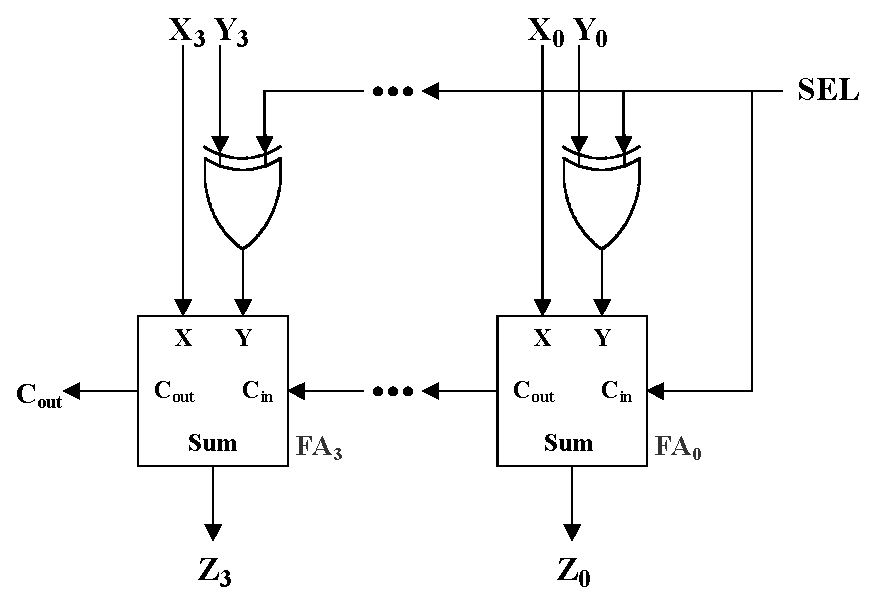
\includegraphics[width=\textwidth]{adder}
%   \caption{\label{fig:adder} 4-bit adder/subtractor.}
% \end{figure}

\begin{table}[hbtp]
  \centering
  \begin{tabular}{c|cc|cc|cc|cc}
 & \multicolumn{2}{c|}{Inputs} & \multicolumn{2}{c|}{PS} & \multicolumn{2}{c|}{NS} & \multicolumn{2}{c}{Outputs} \\
mt    &	EL     & UP & Q1 & Q0    & Q1+ & Q0+ & Z1 & Z0 \\
\hline
0     &	0      & 0  & 0  & 0     &     &     & 0  & 0  \\
1     &	0      & 0  & 0  & 1     &     &     & 0  & 1  \\
2     &	0      & 0  & 1  & 0     &     &     & 1  & 0  \\
3     &	0      & 0  & 1  & 1     &     &     & 1  & 1  \\
4     &	0      & 1  & 0  & 0     &     &     & 0  & 0  \\
5     &	0      & 1  & 0  & 1     &     &     & 0  & 1  \\
6     &	0      & 1  & 1  & 0     &     &     & 1  & 0  \\
7     &	0      & 1  & 1  & 1     &     &     & 1  & 1  \\
8     &	1      & 0  & 0  & 0     &     &     & 0  & 0  \\
9     &	1      & 0  & 0  & 1     &     &     & 0  & 1  \\
10    &	1      & 0  & 1  & 0     &     &     & 1  & 0  \\
11    &	1      & 0  & 1  & 1     &     &     & 1  & 1  \\
12    &	1      & 1  & 0  & 0     &     &     & 0  & 0  \\
13    &	1      & 1  & 0  & 1     &     &     & 0  & 1  \\
14    &	1      & 1  & 1  & 0     &     &     & 1  & 0  \\
15    &	1      & 1  & 1  & 1     &     &     & 1  & 1  \\
\end{tabular}
  \caption{\label{tab:values} }
\end{table}

\section{VHDL}
\label{sec:vhdl}

\begin{verbatim}
library IEEE;
use IEEE.STD_LOGIC_1164.all;
use work.project3_gates.all;

entity circuit is
  port (X    : in  std_logic_vector(3 downto 0);
        Y    : in  std_logic_vector(3 downto 0);
        Z    : out std_logic_vector(3 downto 0);
        SEL  : in  std_logic;
        Cout : out std_logic;
        OVR  : out std_logic);
end circuit;

architecture Structural of circuit is

  signal C : std_logic_vector(3 downto 0);
  signal S : std_logic_vector(3 downto 0);

begin

  x3 : ExclusiveOR port map(SEL, Y(3), S(3));
  x2 : ExclusiveOR port map(SEL, Y(2), S(2));
  x1 : ExclusiveOR port map(SEL, Y(1), S(1));
  x0 : ExclusiveOR port map(SEL, Y(0), S(0));

  fa3 : FullAdder port map(X(3), S(3), C(2), C(3), Z(3));
  fa2 : FullAdder port map(X(2), S(2), C(1), C(2), Z(2));
  fa1 : FullAdder port map(X(1), S(1), C(0), C(1), Z(1));
  fa0 : FullAdder port map(X(0), S(0), SEL, C(0), Z(0));

  Cout <= C(3);
  OVR <= (((not X(3)) and (not Y(3)) and C(3)) or (X(3) and Y(3) and (not C(3))));

end Structural;
\end{verbatim}

\end{document}
